% --- LLM inference: prefill vs.\ decode ---
\begin{frame}{Understanding LLM Inference}
  \begin{columns}[T,onlytextwidth]
    \column{0.52\textwidth}
      \begin{itemize}\footnotesize
        \item[\textcolor{red}{$\blacktriangleright$}] Most popular decoder-only LLMs (e.g., GPT-3) are pretrained for \textbf{causal language modeling}: predicting the next token in a sequence.
        \item[\textcolor{red}{$\blacktriangleright$}] At inference, LLMs receive a series of \textbf{tokens} as input and generate the following tokens \textbf{autoregressively} until a stopping criterion is met\\
          {\scriptsize (e.g., token limit, stop word, or special \texttt{<end>} token).}
        \item[\textcolor{red}{$\blacktriangleright$}] \textbf{Tokens} are about 4 English characters each.
        \item[\textcolor{red}{$\blacktriangleright$}] The inference process has \textbf{two phases}: \textbf{prefill} (process prompt in parallel) and \textbf{decode} (step-by-step token generation).
      \end{itemize}
    \column{0.46\textwidth}
      \centering
      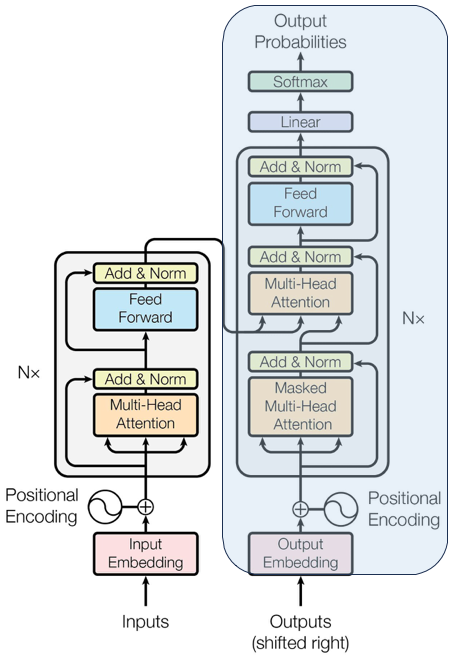
\includegraphics[width=\linewidth,height=0.74\textheight,keepaspectratio]{images/introduction-to-transformers/transformer_variant_decoder_only_alt_highlighted.png}\\[-0.2em]
      {\scriptsize Highlighted: the stack a decoder-only LLM keeps. Vaswani et al., ``Attention Is All You Need,'' \href{https://arxiv.org/abs/1706.03762}{arXiv:1706.03762}, Figure 1.}
  \end{columns}
\end{frame}

\begin{frame}{Prefill Phase: Parallel Input Processing}
  \begin{columns}[T,onlytextwidth]
    \column{0.54\textwidth}
      \begin{itemize}\itemsep0.6em
        \item[\textcolor{red}{$\blacktriangleright$}] \textbf{Prefill phase (input processing):}
          \begin{itemize}\itemsep0.25em
            \item All input tokens are processed together to compute \textbf{keys and values} (attention states) for the prompt.
            \item The entire input sequence is known in advance, enabling a highly parallel \textbf{matrix-matrix} computation that fully uses the GPU's throughput.
          \end{itemize}
        \item[\textcolor{red}{$\blacktriangleright$}] \textbf{Token throughput caveat:}
          \begin{itemize}\itemsep0.25em
            \item Different LLMs may use different \textbf{tokenizers}, so ``tokens per second'' is not always comparable across models, as token-to-character mappings vary.
          \end{itemize}
      \end{itemize}
    \column{0.44\textwidth}
      \centering
      \vspace{1.2em}
      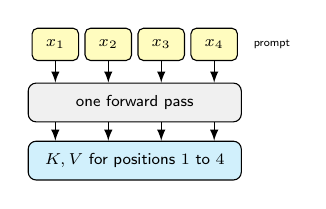
\begin{tikzpicture}[font=\sffamily\scriptsize, >=latex, scale=0.82,
          every node/.style={transform shape},
          tok/.style={draw, fill=yellow!25, minimum width=0.72cm, minimum height=0.5cm, rounded corners=0.07cm},
          pass/.style={draw, fill=gray!12, minimum width=3.3cm, minimum height=0.6cm, rounded corners=0.1cm},
          kvbox/.style={draw, fill=cyan!18, minimum width=3.3cm, minimum height=0.6cm, rounded corners=0.1cm}]
        \foreach \i/\x in {1/0, 2/0.82, 3/1.64, 4/2.46}
          {\node[tok] (t\i) at (\x,1.85) {$x_{\i}$};}
        \node[font=\sffamily\tiny, anchor=west] at (2.95,1.85) {prompt};
        \node[pass] (p) at (1.23,0.95) {one forward pass};
        \node[kvbox] (kv) at (1.23,0.05) {$K,V$ for positions $1$ to $4$};
        \foreach \i in {1,...,4}{\draw[->] (t\i.south) -- (t\i.south |- p.north);}
        \foreach \i in {1,...,4}{\draw[->] (t\i.south |- p.south) -- (t\i.south |- kv.north);}
      \end{tikzpicture}\\[0.4em]
      {\scriptsize All prompt positions are computed in a single pass.}
  \end{columns}
\end{frame}

\begin{frame}{Decode Phase: Serial Token Generation}
  \begin{columns}[T,onlytextwidth]
    \column{0.55\textwidth}
      \begin{itemize}\itemsep0.6em
        \item[\textcolor{red}{$\blacktriangleright$}] \textbf{Decode phase (generating outputs):}
          \begin{itemize}\itemsep0.25em
            \item Output tokens are generated \textbf{one at a time}, each conditioned on all previously generated tokens.
            \item Computation now becomes a \textbf{matrix-vector} operation, less parallelizable and typically \textbf{memory-bound}: moving weights/activations dominates speed, not raw compute.
            \item Optimising decode is crucial: efficient attention, key/value caching, and memory management are ongoing research topics.
          \end{itemize}
      \end{itemize}
    \column{0.45\textwidth}
      \centering
      \vspace{1.2em}
      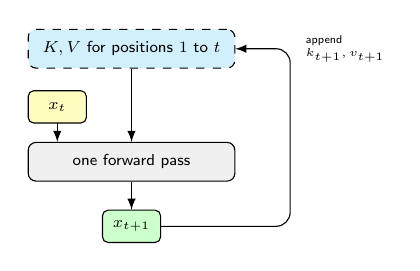
\begin{tikzpicture}[font=\sffamily\scriptsize, >=latex, scale=0.82,
          every node/.style={transform shape},
          tok/.style={draw, fill=yellow!25, minimum width=0.9cm, minimum height=0.5cm, rounded corners=0.07cm},
          new/.style={draw, fill=green!20, minimum width=0.9cm, minimum height=0.5cm, rounded corners=0.07cm},
          cache/.style={draw, dashed, fill=cyan!18, minimum width=3.2cm, minimum height=0.6cm, rounded corners=0.1cm},
          pass/.style={draw, fill=gray!12, minimum width=3.2cm, minimum height=0.6cm, rounded corners=0.1cm}]
        \node[cache] (c) at (0,2.0) {$K,V$ for positions $1$ to $t$};
        \node[tok] (xt) at (-1.15,1.1) {$x_t$};
        \node[pass] (p) at (0,0.25) {one forward pass};
        \node[new] (xn) at (0,-0.75) {$x_{t+1}$};
        \draw[->] (c.south) -- (p.north);
        \draw[->] (xt.south) -- (xt.south |- p.north);
        \draw[->] (p.south) -- (xn.north);
        % Feedback edge: the pass appends its own K,V and the new token re-enters as input.
        \draw[->, rounded corners=0.18cm] (xn.east) -- ++(2.0,0) |- (c.east)
          node[midway, anchor=west, font=\sffamily\tiny, align=left, xshift=0.12cm] {append\\$k_{t+1},v_{t+1}$};
      \end{tikzpicture}\\[0.4em]
      {\scriptsize One position per pass; the cache grows every step.}
  \end{columns}
\end{frame}


\begin{frame}{Why Optimise Inference?}
  \begin{itemize}
    \item[\textcolor{red}{$\blacktriangleright$}] \textbf{Training} is often one-off; \textbf{inference} is repeated at scale (cost, latency, energy).
    \item[\textcolor{red}{$\blacktriangleright$}] Large language models are \textbf{memory-bound} and \textbf{autoregressive}: each new token revisits all previous tokens.
    \item[\textcolor{red}{$\blacktriangleright$}] Goals: lower \textbf{latency} (interactive UX), higher \textbf{throughput} (serving many users), smaller \textbf{memory} (long contexts, edge).
  \end{itemize}
\end{frame}

\begin{frame}{Measuring Inference}
  \begin{itemize}\itemsep0.5em
    \item[\textcolor{red}{$\blacktriangleright$}] \textbf{Time to first token (TTFT):} how long until the first output token appears; set by the prefill phase, which is compute-bound.
    \item[\textcolor{red}{$\blacktriangleright$}] \textbf{Time per output token (TPOT):} the gap between subsequent tokens; set by the decode phase, which is memory-bound.
    \item[\textcolor{red}{$\blacktriangleright$}] Request latency $\approx$ TTFT $+$ TPOT $\times$ number of generated tokens.
    \item[\textcolor{red}{$\blacktriangleright$}] \textbf{Throughput:} total tokens per second across all requests. Batching raises throughput but can hurt per-request latency; serving systems balance the two.
  \end{itemize}
\end{frame}
